\section{Master's Project: Design Decisions}

\subsection{Initial Plan}
Despite the many areas of improvement for our senior project, we initially believed that a functional tester was adequate for most student-designed VLSI chips. It is worth noting that at the time of our senior project semester, students in VLSI designed their chips using a 0.6 micron process. Generally, chips fabricated using this process cannot run beyond 25 MHz. As such, we believed the best course of action was to polish our system (e.g. simplify the user interface and setup) in order to allow students to test their chips' functionality. For any timing-sensitive chips, students would be advised to construct a development board for their chip and use a logic analyzer or oscilloscope to analyze signals in detail.

When we first proposed expanding upon our senior project for our Master's project, our basic plan was to do the following: 
\begin{itemize}
\item Eliminate the Numato Saturn and fabricate a MOSIS chip containing the finite state machine logic originally used by the Saturn.
\item Replace the double-buffered shift registers inside the Saturn with external double-buffered shift registers controlled by a MOSIS chip.
\item Implement autoschmooing by replacing the trimpot on our variable voltage regulator with a digital pot.
\item Expand upon our C Sharp program (e.g. create schmooing plots).
\item Try to redesign our main PCB with equilibrium tracing.
\end{itemize}

While the plan seemed solid at first, we quickly became concerned that the project may not have been challenging enough for a Master's project. We soon came to believe that attempting to implement both autoschmooing and real-time testing would provide a more suitable challenge to us, and so, we decided to revamp our entire senior project design.

\subsection{Revised Plan}
We redefined the goals of our Master's project as follows: 
\begin{itemize}
\item Simpler interface and setup. Ideally, the entire system would be plug-and-play.
\item Real-time testing (where a test cycle is executed immediately following completion of the preceding test cycle).
\item Timing information (via PCB equilibrium tracing).
\item Automated schmooing.
\item More test cycle configurations.
\end{itemize}

We spent Fall 2015 brainstorming ideas to implement the above goals. We proposed the schematic in Figure \ref{fig:f15_schematic} at the end of the semester. Below, we detail each major component of this schematic.

\begin{figure}
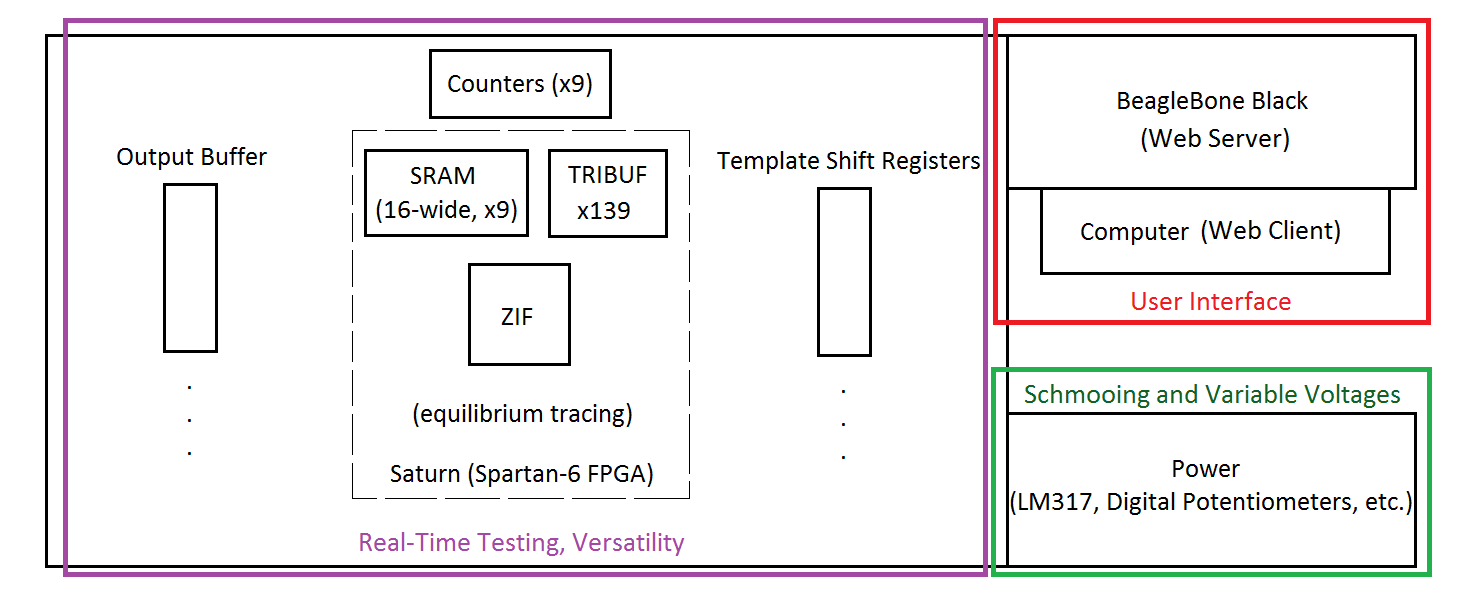
\includegraphics[width=1.0\textwidth]{original_schematic.png}
\caption{Schematic proposed at end of Fall 2015 semester.}
\label{fig:f15_schematic}
\end{figure}

\subsubsection{User Interface}
With our senior project, the user needed to use Windows in order to run our GUI and had to program MicroBlaze every time the system lost power. With our Master's project, we wanted a "plug and play" interface. To eliminate the need for any particular OS, we decided to use a web browser to interface with the testing system. We decided to use the BeagleBone Black board that Norm and Daniel each purchased when they took Advanced Embedded Software in Fall 2014.

The BeagleBone Black works well because it can host a small web server, runs on Linux, has the necessary I/O (SPI, UART, GPIO), and provides plenty of memory. 

\subsubsection{Timing and Voltage Schmooing}
Time schmooing, i.e. modulating the test cycle configuration (delay, width, length) between tests, naturally requires equilibrium tracing. We planned to manually route any PCBs we would design to minimize the difference in trace lengths.

Figure \ref{fig:power_schematic} is a schematic that we designed for voltage schmooing. Much of the schematic is based upon the variable voltage regulator LM317's datasheet. As the LM317 uses a reference voltage of 1.25V, we added a -1.25V bias created by an op-amp buffer (bottom-left of schematic) to set the reference voltage to 0V. We learned of this trick from  \href{http://electronics.stackexchange.com/questions/186760/why-do-linear-voltage-regulators-have-minimum-output-voltage-0-v}{this} StackExchange post. 

\begin{figure}[!h]
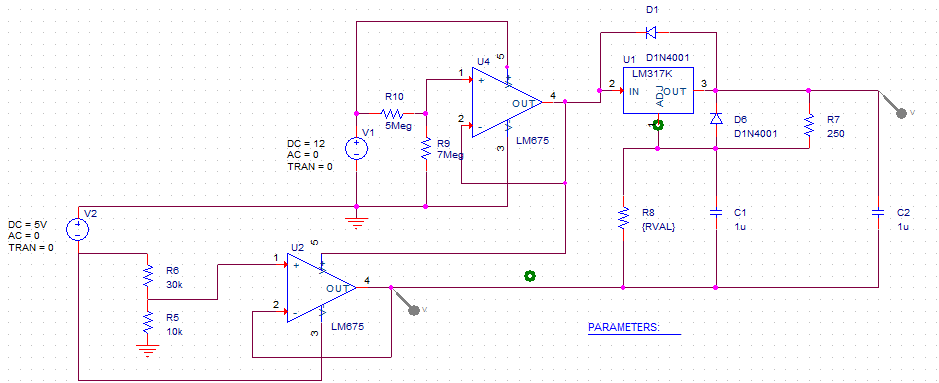
\includegraphics[width=1.0\textwidth]{power_schematic.png}
\caption{Power schematic for voltage schmooing.}
\label{fig:power_schematic}
\end{figure}

We simulated this schematic in PSpice and prototyped the schematic using a trimpot for the variable resistor. Figure \ref{fig:power_results} shows that the output voltage, much to our liking, responds linearly to a change in the resistance of the variable resistor.

There is an important tradeoff worth mentioning with this schematic. A higher variable resistor allows for more granularity in the output voltage. However, there is a small but fixed current that travels through the variable resistor; a larger variable resistor creates a larger error term in the output voltage. Refer to the LM317's datasheet online for more information.

For the variable resistor, we researched digital potentiometers and found that the AD5293, with 10-bit resolution at 20 kOhms, should serve well for the project.

\begin{figure}
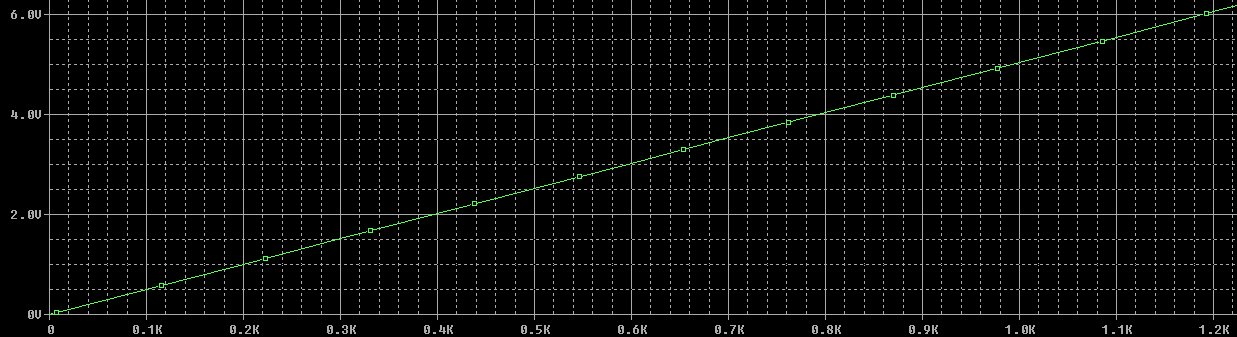
\includegraphics[width=1.0\textwidth]{power_results.png}
\caption{PSpice simulation results for power circuitry.}
\label{fig:power_results}
\end{figure}

\subsubsection{Real-Time Testing}
Devising a plan for real-time testing was easily the most challenging issue we faced. With our senior project, handling one input and output vector at a time was convenient because we only needed one set of double-buffered registers for all of the vectors associated with a test cycle. As such, we had to determine where the input vectors and output vectors should actually be stored.

Ultimately, we proposed the scheme in Figure \ref{fig:real_time_testing}. The basic idea was to store output vectors into external SRAM chips, and then later fetch the SRAM contents using some sort of parallel-to-serial shift register. Not shown in the image, we chose to store the input vectors in the Spartan-6 FPGA's block RAM (which allow for fast reads).

The key idea is that during test execution -- the only moment in which timing is important as far as the DUT goes -- the system only concerns itself with fetching and applying input vectors. 

\begin{figure}
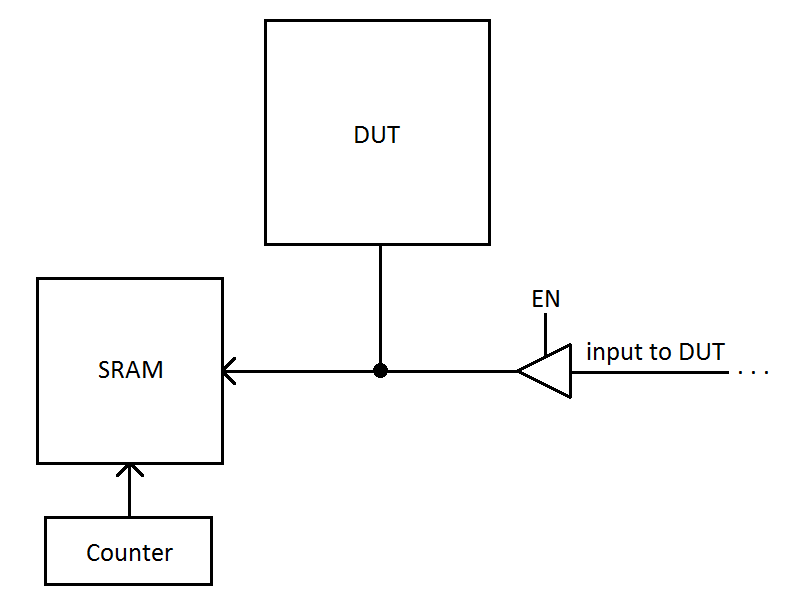
\includegraphics[width=1.0\textwidth]{real_time_testing.png}
\caption{Real-time testing scheme. Input vectors are stored in the FPGA's block RAM; output vectors are stored in separate SRAM chips.}
\label{fig:real_time_testing}
\end{figure}

\subsubsection{Versatility}
Though we had no specific proposals at the end of Fall 2015, we hoped to bring legacy to our project and make it upgradeable and adequate for students to use for at least a few years.

Ultimately, some of the ways we encompassed versatility in our project design is the use of multiple PCBs and the BeagleBone Black web server, which is easy to develop on.

\newpage